\section{Description et justification de la structure fonctionnelle}

\subsubsection*{Objectifs}

Cette section présente l'organisation du système en blocs fonctionnels et décrit leurs 
interactions. Chaque bloc (réception de trame, FIFO, registre d'état, interface microprocesseur) 
est expliqué dans son rôle et sa contribution au fonctionnement global. L'objectif est de montrer 
comment les fonctionnalités spécifiées sont réparties de manière logique pour répondre au cahier 
des charges.
\newline

Dans cette section, nous établissons une structure fonctionnelle indépendante de la technologie.

\begin{figure}[H]
    \centering
    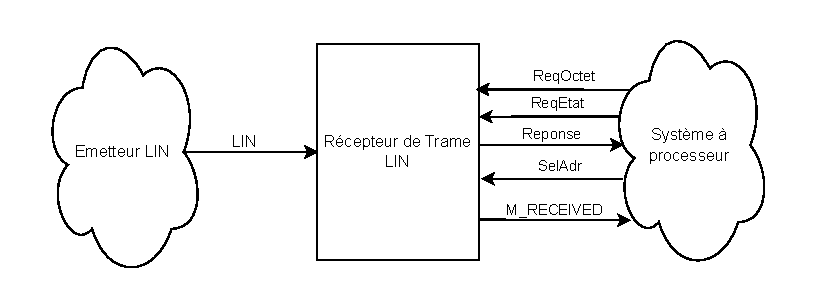
\includegraphics[width=0.8\linewidth]{images/inter/Structure_Fonc_Circuit.pdf}
    \caption{Structure fonctionnelle du système}
    \label{fig:placeholder}
\end{figure}

Pour le moment, nous nous sommes limités à deux blocs principaux : l'interface microprocesseur et 
la réception des trames. Ces deux blocs sont connectés à un bloc d'échange, qui permet la 
communication entre eux. Ce bloc assure l'interprétation des échanges avec le microprocesseur ainsi 
que la gestion des deux registres de données.
\newline

% page 12
\begin{figure}[H]
    \centering
    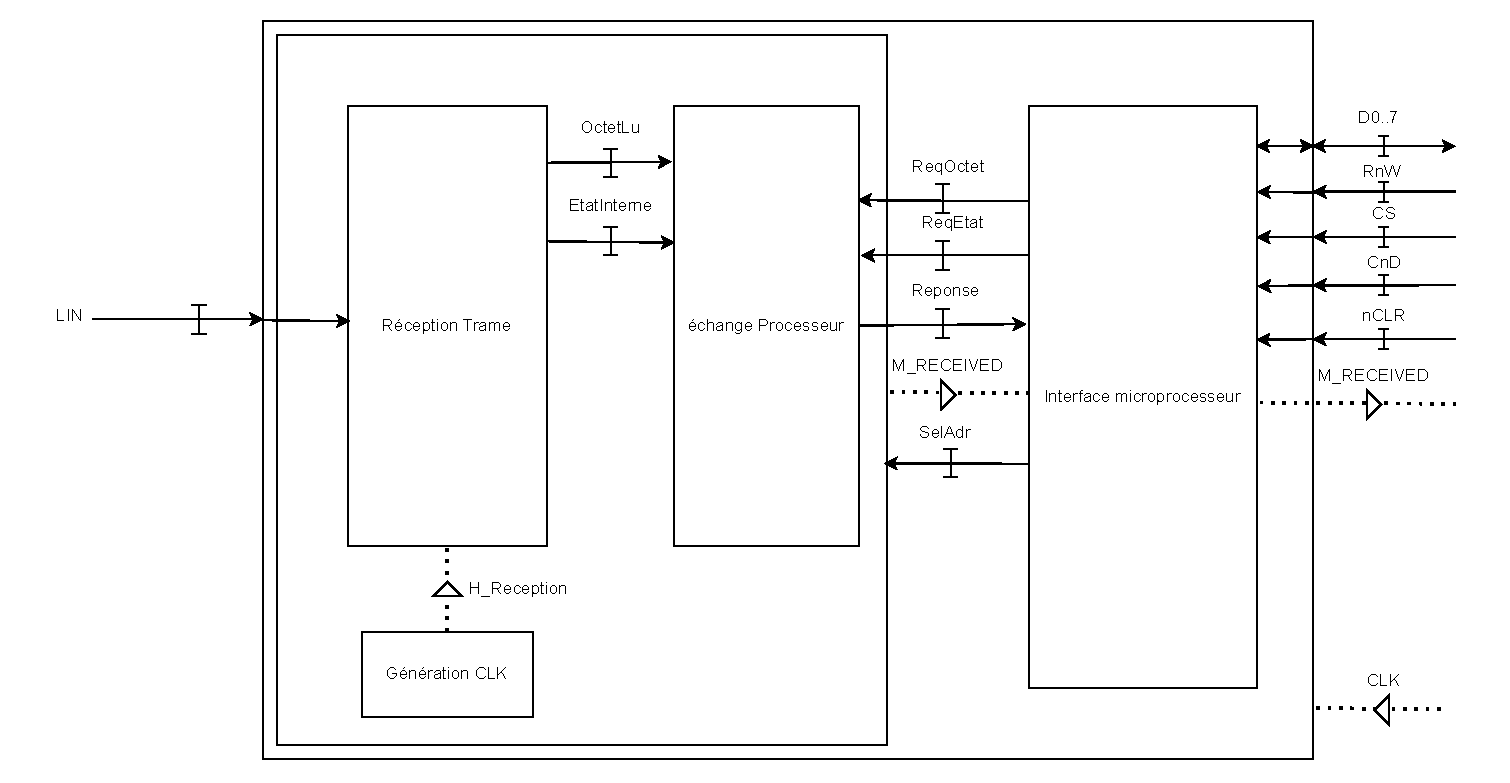
\includegraphics[width=0.8\linewidth]{images/inter/Schema_base_circuit.pdf}
    \caption{Architecture du système de réception de trame LIN V1}
    \label{fig:placeholder}
\end{figure}

Nous pouvons également représenter l'automate du système de communication avec le processeur : 

\begin{figure}[H]
    \centering
    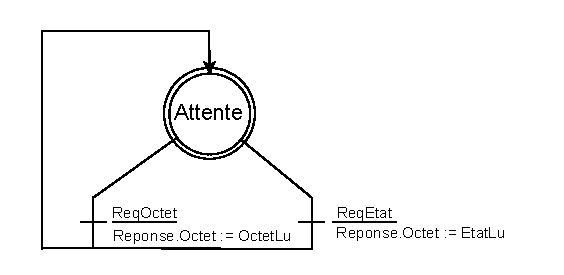
\includegraphics[width=0.8\linewidth]{images/inter/Echange_Processeur.pdf}
    \caption{Échanges avec le processeur}
    \label{fig:placeholder}
\end{figure}


Dans notre démarche d'optimisation du système, nous nous sommes rendu compte que le bloc d'échange 
microprocesseur pouvait être intégré au bloc d'interface. Cela permettra de supprimer des signaux 
supplémentaires, inutiles et encombrants.
\newline

%page 13
\begin{figure}[H]
    \centering
    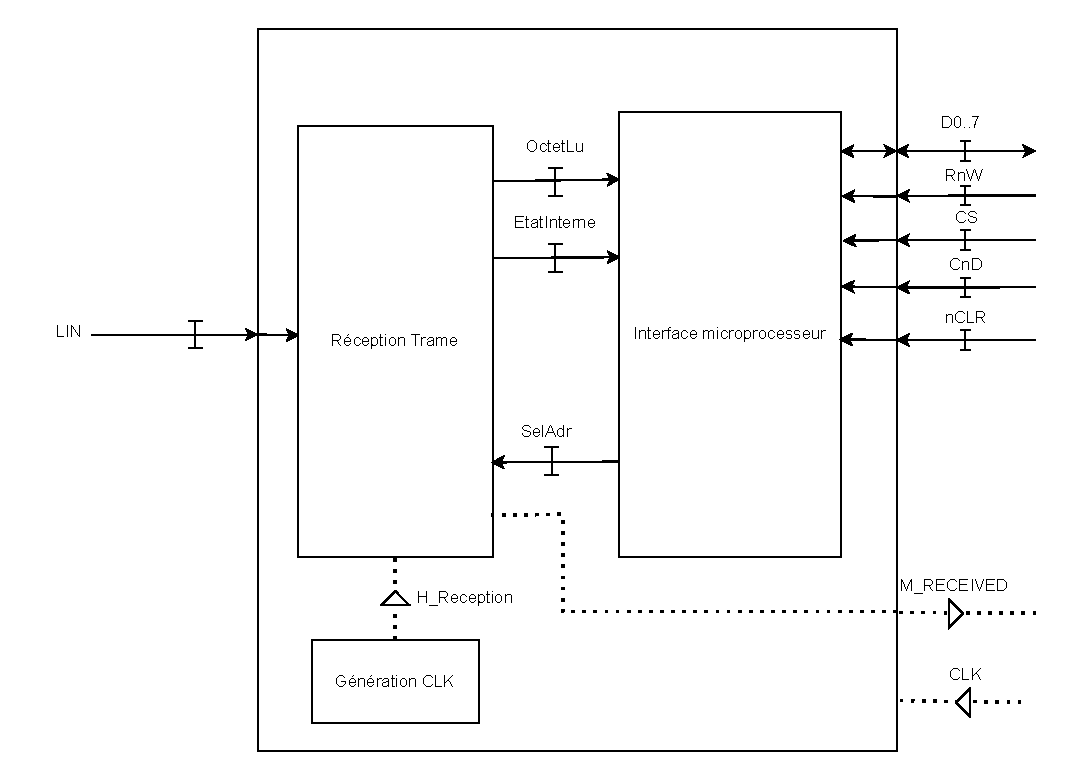
\includegraphics[width=0.8\linewidth]{images/inter/Schema_avance_circuit.pdf}
    \caption{Architecture du système de réception de trame LIN V2}
    \label{fig:placeholder}
\end{figure}

Par la suite, nous avons décidé d'ajouter deux blocs de registres internes : le registre de stockage 
des données de la trame LIN (FIFO) et le registre d'état interne (ETAT), qui permet de connaître les 
informations sur l'état de la réception.
\newline

%page 16
\begin{figure}[H]
    \centering
    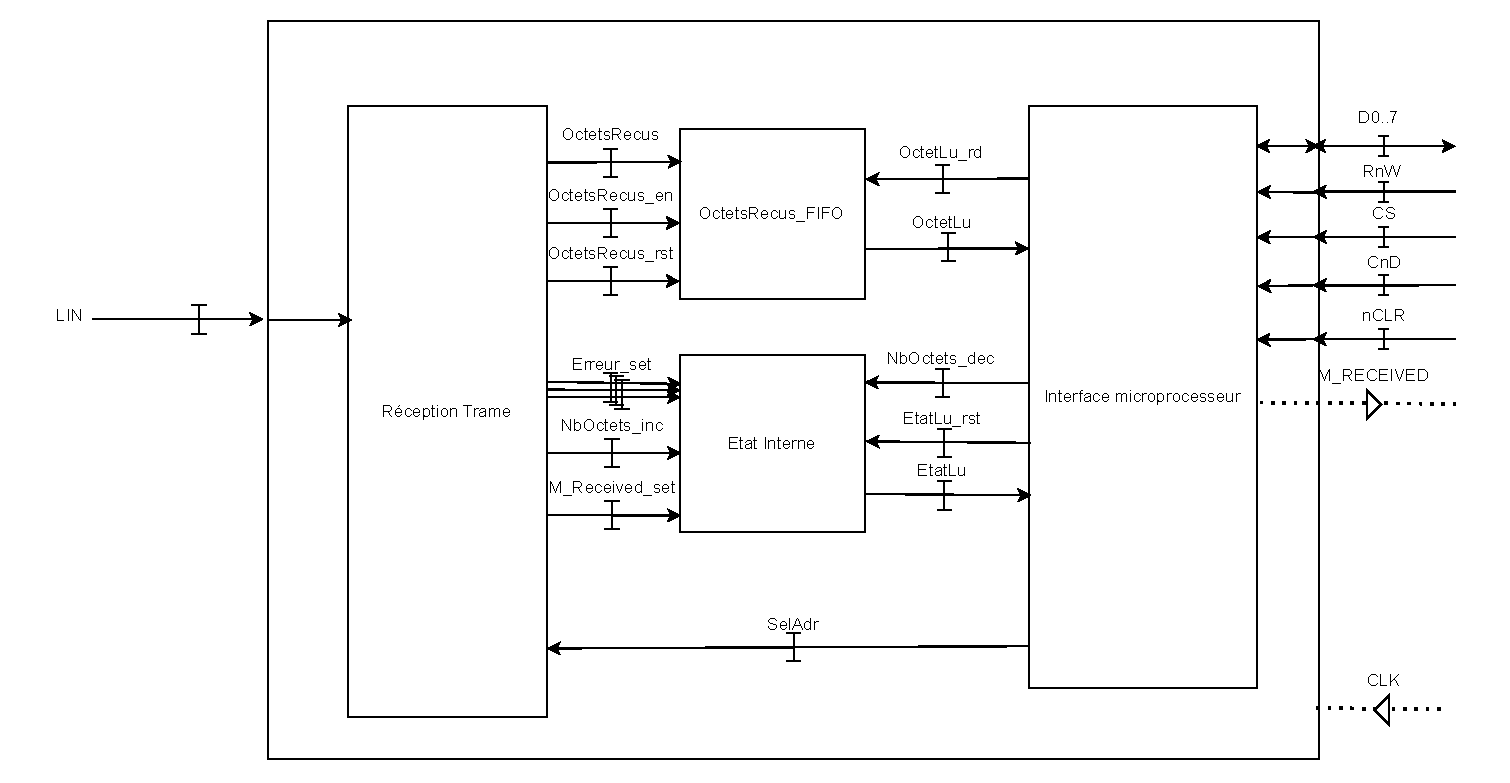
\includegraphics[width=0.8\linewidth]{images/inter/Schema_Final.pdf}
    \caption{Description finale du circuit}
    \label{fig:placeholder}
\end{figure}

Comme indiqué ci-dessus, dans le schéma de notre système global, nous avons décidé d'ajouter 
certains signaux internes entre les blocs de registres et les interfaces.
\newline

\subsubsection*{FIFO}

\begin{center}
\renewcommand{\arraystretch}{1.2} % espace vertical
\small % pour uniformiser la taille du texte
    \begin{tabularx}{\textwidth}{|c||c|c|X|}
     \hline			
       \textbf{Signaux} & \textbf{Mode} & \textbf{Type} & \textbf{Description}  \\ \hline 
       OctetRecu\_WR & IN & \texttt{STD\_LOGIC} & Read / Write opération \\
       OctetRecu\_RST & IN & \texttt{STD\_LOGIC} & Réinitialisation des données reçue \\
       OctetLu\_RD & IN & \texttt{STD\_LOGIC} & Sélection de la mémoire (Control / Data) \\
     \hline  
    \end{tabularx}
\end{center}

La définition de ces nouveaux signaux permet de gérer de manière précise le fonctionnement de la 
FIFO. OctetRecu\_WR est un signal d'écriture qui déclenche l'enregistrement d'un octet reçu dans 
la mémoire FIFO, garantissant que chaque donnée entrante est correctement stockée. OctetRecu\_RST 
est un signal de réinitialisation qui vide complètement la FIFO et remet à zéro tous les compteurs 
internes, permettant ainsi de reprendre la réception de données sans risque de corruption ou de 
chevauchement. OctetLu\_RD est un signal de lecture qui active l'accès aux données stockées dans 
la FIFO et permet leur transfert vers le microprocesseur ou d'autres blocs du système. Ensemble, 
ces signaux assurent une communication fiable, synchronisée et organisée entre l'interface 
microprocesseur et le registre de réception, tout en facilitant la gestion des flux de données 
entrants.
\newline

\subsubsection*{ETAT}

\begin{center}
\renewcommand{\arraystretch}{1.2} % espace vertical
\small % pour uniformiser la taille du texte
    \begin{tabularx}{\textwidth}{|c||c|c|X|}
     \hline			
       \textbf{Signaux} & \textbf{Mode} & \textbf{Type} & \textbf{Description}  \\ \hline 
       NbOctetRecu\_RST & IN & \texttt{STD\_LOGIC} & Réinitialisation du compteur d'octets \\
       DecNbOctet & IN & \texttt{STD\_LOGIC} & Flag de lecture pour FIFO \\
       EtatLu\_RST & IN & \texttt{STD\_LOGIC} & Reset de l'état lu \\
     \hline  
    \end{tabularx}
\end{center}

La définition de ces signaux du bloc ETAT permet de contrôler et de suivre l'état interne de la 
réception des données. NbOctetRecu\_RST réinitialise le compteur d'octets reçus, assurant un 
suivi précis du nombre de données traitées. DecNbOctet agit comme un indicateur de lecture pour 
la FIFO, signalant quand un octet peut être lu et transféré, ce qui permet une gestion correcte 
des flux de données. EtatLu\_RST permet de réinitialiser les informations d'état lues, garantissant 
que le système dispose toujours d'une représentation exacte de l'état actuel de la réception. 
Ensemble, ces signaux assurent une supervision fiable et synchronisée des opérations internes, 
facilitant le contrôle et la gestion du flux de données dans le système.
